\subsection{Calibrating distance modulus from $E_{peak}-E_{gamma}$ relation}
Having luminosity correlations calibrated, we can conversely using these correlations to calibrate the distance of GRBs, and further use GRBs to constrain cosmological models. Since our calibration of luminosity correlations is independent of cosmological model, the circularity problem is avoided. As we have seen, the $E_{p}-E_{\gamma}$ relation is not significantly evolving with redshift, so we use this relation to calibrate the distance of GRBs. Due to that the TABLE 1
\begin{figure}[H]
	\centering
	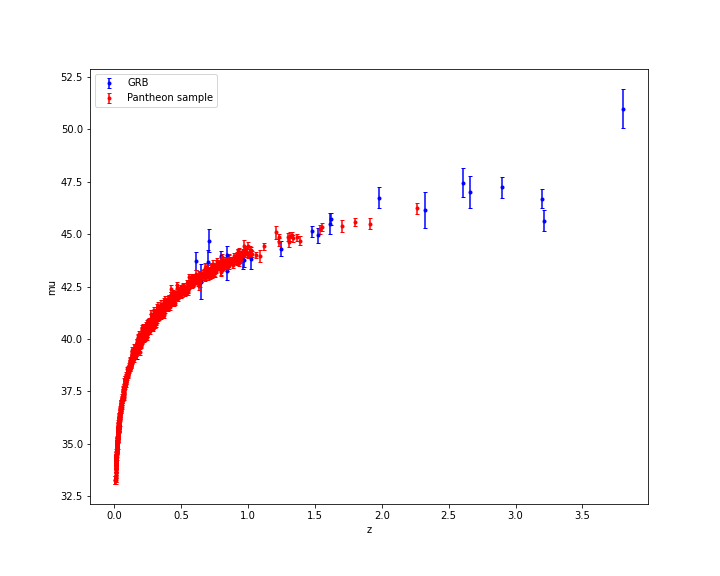
\includegraphics[width=0.7\textwidth]{pantheon/gp/16_GRB_reconstruction.png}
	\caption{GRB Hubble Diagram}
	\label{fig:HD_GRB_GP}
\end{figure}